%%%%%%%%%%%%%%%%%%%%%%%%%%%%%%%%%%%%%%%%%%%%%%%%%%%%%%%%%%%%%%%%%%%%%%%
%% AGI-22 paper about temporal and procedural reasoning with OpenCog %%
%%%%%%%%%%%%%%%%%%%%%%%%%%%%%%%%%%%%%%%%%%%%%%%%%%%%%%%%%%%%%%%%%%%%%%%

\documentclass[runningheads]{llncs}
%
\usepackage{graphicx}
\usepackage{amsmath}
\usepackage{amssymb}
\usepackage{bussproofs}
\usepackage{cite}
\usepackage{wrapfig}
\usepackage{sidecap}

% For ⩘ and ⩗ (requires the LuaLaTeX engine)
\usepackage{unicode-math}
\setmathfont{Stix Two Math}

% Commands for Atomese code
\newcommand{\SP}{\;\;\;}
\newcommand{\TTrue}{\textit{True}}
\newcommand{\TFalse}{\textit{False}}
\newcommand{\TAtom}{\textit{Atom}}
\newcommand{\TTime}{\textit{Time}}
\newcommand{\TEval}{\textit{Evaluation}}
\newcommand{\TList}{\textit{List}}
\newcommand{\TLamb}{\textit{Lambda}}
\newcommand{\TExec}{\textit{Execution}}
\newcommand{\TAtTime}{\textit{AtTime}}
\newcommand{\TAnd}{\textit{And}}
\newcommand{\TOr}{\textit{Or}}
\newcommand{\TNot}{\textit{Not}}
\newcommand{\TImpl}{\textit{Implication}}
\newcommand{\TPredImpl}{\textit{PredictiveImplication}}
\newcommand{\TSeqAnd}{\textit{SequentialAnd}}
\newcommand{\TSeqOr}{\textit{SequentialOr}}
\newcommand{\TBSeqAnd}{\textit{BackSequentialAnd}}
\newcommand{\TFSeqAnd}{\textit{ForeSequentialAnd}}
\newcommand{\TLag}{\textit{Lag}}
\newcommand{\TLead}{\textit{Lead}}
\newcommand{\TTV}{\textit{TV}}
\newcommand{\TTVPi}{\textit{TV}_i^P}
\newcommand{\TTVQi}{\textit{TV}_i^Q}
\newcommand{\TTVP}{\textit{TV}^P}
\newcommand{\TTVQ}{\textit{TV}^Q}
\newcommand{\TTVR}{\textit{TV}^R}
\newcommand{\TTVPQ}{\textit{TV}^{PQ}}
\newcommand{\TTVQR}{\textit{TV}^{QR}}
\newcommand{\TBTV}{\langle \TTV \rangle}
\newcommand{\TBTVPi}{\langle \TTVPi \rangle}
\newcommand{\TBTVQi}{\langle \TTVQi \rangle}
\newcommand{\TBTVP}{\langle \TTVP \rangle}
\newcommand{\TBTVQ}{\langle \TTVQ \rangle}
\newcommand{\TBTVR}{\langle \TTVR \rangle}
\newcommand{\TBTVPQ}{\langle \TTVPQ \rangle}
\newcommand{\TBTVQR}{\langle \TTVQR \rangle}
\newcommand{\Tstrength}{\textit s}
\newcommand{\Tconf}{\textit c}

% Commands for symbolic mathematical notations
\newcommand{\prob}{\mathbf{Pr}}
\newcommand{\limp}{\rightarrow}
\newcommand{\lpreimp}[1]{\leadsto^{#1}}
\newcommand{\lseqor}[1]{\!\bigslopedvee^{#1}\!}
\newcommand{\lseqand}[1]{\!\bigslopedwedge^{#1}\!}
\newcommand{\ldo}[1]{\widehat{#1}}
\newcommand{\llag}[2]{\overrightarrow{#1}^{#2}}
\newcommand{\llead}[2]{\overleftarrow{#1}^{#2}}
%% TODO: try to replace over right arrow by over right harp, etc
%% \newcommand{\llag}[2]{\accentset{\overrightharp}{#1}^{#2}}
%% \newcommand{\llead}[2]{\overleftharp{#1}^{#2}}

% Commands for schemata vocabulary
\newcommand{\lgo}[1]{\textit{go}(#1)}

\begin{document}
%
\title{Rational OpenCog Controlled Agent}

%\titlerunning{Abbreviated paper title}
% If the paper title is too long for the running head, you can set
% an abbreviated paper title here
%
\author{Nil Geisweiller
  %\orcidID{0000-0001-5041-6299}
  \and Hedra Yusuf}
%
\authorrunning{N. Geisweiller et al.}
% First names are abbreviated in the running head.
% If there are more than two authors, 'et al.' is used.
%
\institute{ SingularityNET Foundation, The
  Netherlands\\ \email{\{nil,hedra\}@singularitynet.io}}
%
\maketitle              % typeset the header of the contribution
%

\begin{abstract}
  In this paper we introduce, ROCCA for \emph{Rational OpenCog
    Controlled Agent}, an agent, that, as its name suggests, attempts
  to leverage the OpenCog framework to acts rationally in uncertain
  environments by relying on reasoning all the way, from learning to
  planning.  An experiment in a Minecraft environment is provided as a
  test case.

  \keywords{
    Symbolic Reinforcement Learning \and
    Pattern Mining \and
    Procedural Reasoning \and Thompson Sampling \and OpenCog \and
    Minecraft}
\end{abstract}

\section{Introduction}
This paper describes an attempt to leverage the OpenCog
framework~\cite{Hart2008} for controlling agents in uncertain
environments.  It can be seen as a reboot of previous
attempts~\cite{Goertzel2008, Goertzel2011CSP, Cai2013}
relying on new or improved components such as
\begin{itemize}
\item a hypergraph pattern miner~\cite{Geisweiller2019} and a version
  of PLN~\cite{Goertzel2009} both implemented on top of OpenCog's
  Unified Rule Engine equipped with an inference control mechanism;
\item a temporal and procedural extension of
  PLN~\cite{Geisweiller2023TPLN};
\item a simplified version of OpenPsi~\cite{Cai2013} leaving
  aside built-in urges and modulators from MicroPsi~\cite{Bach2012}
  and using an action selection policy based on Thompson
  Sampling~\cite{Leike2016}.
\end{itemize}
It is comparable to OpenNARS for Applications (ONA)~\cite{Hammer2020}
but, among other differences, uses PLN~\cite{Goertzel2009} as its core
logic.
% rather than NAL~\cite{Wang2011}.

The ultimate goal of this project is to provide a technology to enable
us to experiment with forms of meta-learning and introspective
reasoning for self-improvements.  The rational for using a
reasoning-based system is that it offers maximum transparency and is
thus more amenable to reflectivity and
introspection~\cite{Schmidhuber2003, Goertzel2014EGI1}.  The work that
is described in this paper is only the premise of that goal.  No
meta-learning is taking place yet.  The objective for now is to build
an agent that is able to discover regularities from its environment
and acts rationally, possibly at the expense of efficiency, at least
initially.  For discovering regularities, the agent uses a
reasoning-based pattern miner~\cite{Geisweiller2019}.  Then combine
these regularities to form plans using temporal and procedural
reasoning.  More specifically plans are predictive implications of the
form
$$C \land A \lpreimp{T} G \measeq \textit{TV}$$
called \emph{Cognitive Schematics} or \emph{Schemata}.  Which can be
read as \emph{``in some context $C$, if some, possibly composite,
  action $A$ is executed, then after $T$ time units, the goal $G$ is
  likely to be fulfilled, with second order probability measured by
  $\textit{TV}$''}.  These plans are then combined to into a mixture
that grossly approximates Solomonoff
distribution~\cite{Geisweiller2018}.  Finally, the next action is
selected using Thompson Sampling~\cite{Leike2016}.  The resulting
system is called ROCCA for \emph{Rational OpenCog Controlled Agent}.

% But before to make an agent as rational as possible, not necessarily as
% efficient as possible.  This stems from the concern that in order to
% autonomously gain efficiency the agent must first be able to make the
% best possible decisions, starting first in the outer world, and then
% in the inner world.

% Inner actions could be as transitory as bringing a piece of
% knowledge to the attentional focus, and as profound as rewriting a
% part of its code, like a Goedel Machine.  The atomspace can be
% viewed as a very compact representation of an envelop over
% environments (cite partial operator induction paper).  And PLN can
% be viewed as an abstract-enabling way to calculate the cumulative
% reward (in case it is used as a re-inforcement learner) to be
% maximized, or a goal driven agent in a more general case.  For these
% reasons ROCCA may well be seen as an approximated combination of
% AI\Xi and a Goedel Machine.

% The paper presents

% The agent starts in a completely unknown environment

% The idea is that reasoning is used at all levels, discovering patterns
% from raw observations, building plans and making decisions.

% It is a work in progress.

% Neural networks are excellent at interpolation, but are rather poor at
% extrapolation, what we need for true intelligence is a system that
% thinks critically.

% Rarely do causes and effects take place over arbitrary temporal
% scales.  For instance it is unlikely to find a cause that may produce
% the same effect, or an effect at all, after 1ms, 1 century or any time
% in between.  For that reason we focus on a real time temporal logic.

% \subsection{Related Work}

% ROCCA is essentially a reboot of~\cite{Goertzel2011} using a
% modernized version of the OpenCog pattern miner, as well as a
% simplified version of OpenPsi~\cite{Cai2011, Cai2013} leaving aside
% various built-in urges and modulators from MicroPsi~\cite{Bach2012}
% and using an action selection policy based on Thompson
% Sampling~\cite{Leike2016}.

% \subsection{Contributions}

% The contributions of that paper are:
% \begin{enumerate}
% \item Design an architecture for controlling an agent based on that
%   temporal reasoning extension.
% \end{enumerate}

The rest of the paper is organized as follows.  A recall of the
OpenCog framework is provided in Section~\ref{sec:opencog}.  ROCCA is
described in Section~\ref{sec:rocca}.  An experiment using it to
control an agent in Minecraft is described in
Section~\ref{sec:minecraft}.  A conclusion including future directions
is given in Section~\ref{sec:conclusion}.
% \subsection{Outline}

% \begin{enumerate}
% \item ROCCA
% \item Minecraft experiment
% \end{enumerate}

\section{OpenCog Framework Recall}
\label{sec:opencog}
OpenCog~\cite{Hart2008} is a framework offering a hypergraph database
technology with a query language and a collection of programs built on
top of it to perform cognitive functions such as learning, reasoning,
spreading attention and more.  Knowledge is stored in
\emph{AtomSpaces}, hypergraphs composed of \emph{atoms}, \emph{links}
and \emph{nodes}, where links can connect to other atoms.
\emph{Values} can be attached to atoms to hold probability,
confidence, importance and more.  Values and atoms can be of various
types.  Let us recall the types we need for the rest of paper.
\begin{itemize}
\item A \emph{TruthValue} is a second order probability distribution,
  i.e. a probability of a probability.
\item A \emph{SimpleTrueValue} is a TruthValue where the second order
  distribution is represented by a beta distribution of parameters
  controlled by a \emph{strength}, a proxy for a probability, and a
  \emph{confidence} over that strength.  It is denoted $<\!s, c\!>$ where
  $s$ is the strength and $c$ is the confidence.
\item A \emph{Predicate} is function from a certain domain to
  $Boolean$.  A TruthValue can be attached to a predicate,
  representing the prevalence of its satisfied inputs.  For instance
  $P \measeq\ <\!0.4, 0.1\!>$ represents that $P$ tends to evaluate to
  $\TTrue$ 40\% of the time, but there is a small confidence of 0.1
  over that 40\%.  A TrueValue can be attached to individual
  evaluations as well.  For instance $P(a) \measeq\ <\!0.9, 1\!>$
  represents that the probability of $P(a)$ evaluating over a
  particular $a$ to $\TTrue$, is 0.9 and we are certain about it.
\item A \emph{Conjunction} is a link between two predicates,
  representing the predicate resulting from the pointwise conjunction
  of these two predicates.  For instance
  $P \land Q \measeq\ <\!0.2, 0.3\!>$ represents the prevalence, with
  strength 0.2 and confidence 0.3, of the pointwise conjunction of $P$
  and $Q$.
\item An \emph{Implication} is a link between two predicates,
  semantically representing the conditional probability between two
  events represented by these predicates.  For instance
  $P \limp Q \measeq\ <\!0.7, 0.4\!>$ indicates that if $P(x)$ is
  $\TTrue$ then there is a 70\% change with a 0.4 confidence,
  that $Q(x)$ is also $\TTrue$.
\end{itemize}
Additionally we use the following types for temporal reasoning.
\begin{itemize}
\item A \emph{Sequential Conjunction} is a link between two temporal
  predicates, representing the predicate resulting from the pointwise
  conjunction of these predicates while the second one leads by a
  certain time.  For instance $P \lseqand{T} Q$ is the pointwise
  conjunction of $P$ and a leading $Q$ by $T$ time units.  Meaning
  that $(P \lseqand{T} Q)(x, t)$ is $\TTrue$ if and only if $P(x, t)$
  and $Q(x, t+T)$ are $\TTrue$.
\item A \emph{Predictive Implication} is a link between two temporal
  predicates, representing the conditional probability between two
  events delayed by a certain time.  For instance
  $P \lpreimp{T} Q \measeq\ <\!0.8, 0.5\!>$ indicates that if $P(x)$
  is $\TTrue$ then there is a 80\% chance with a 0.5 confidence, that
  after $T$ time units $Q(x)$ will also be $\TTrue$.
\end{itemize}
The difference between a temporal and an atemporal predicate is its
domain.  A temporal predicate must have at least a temporal dimension.
% respecting certain properties such as having a total order.
More detail about the temporal types and their associated inference
rules is provided in~\cite{Geisweiller2023TPLN}.

% that query and modify one or several atomspaces. There is an
% overhaul remaking of OpenCog called Hyperon, but we will not touch
% upon that in that paper as ROCCA is built on top of what we may call
% OpenCog Classic,
% % ~\footnote{OpenCog Classic is still
% %   and will remain in development for the foreseeable future}
% the predecessor of Hyperon.
\section{Rational OpenCog Controlled Agent}
\label{sec:rocca}
ROCCA is implemented as an observation-planning-action loop
interleaved with learning and reasoning.  It provides an interfacing
between OpenCog and environments such as Malmo \cite{Johnson2016} or
OpenAI Gym \cite{Brockman2016}.  It is written in Python which is both
supported by these environments and OpenCog.  Figure~\ref{fig:rocca}
provide a graphical representation of ROCCA as if it was a single loop
incorporating all steps.
\begin{wrapfigure}{l}{0.53\textwidth}
  \vspace{10pt}
  \begin{center}
    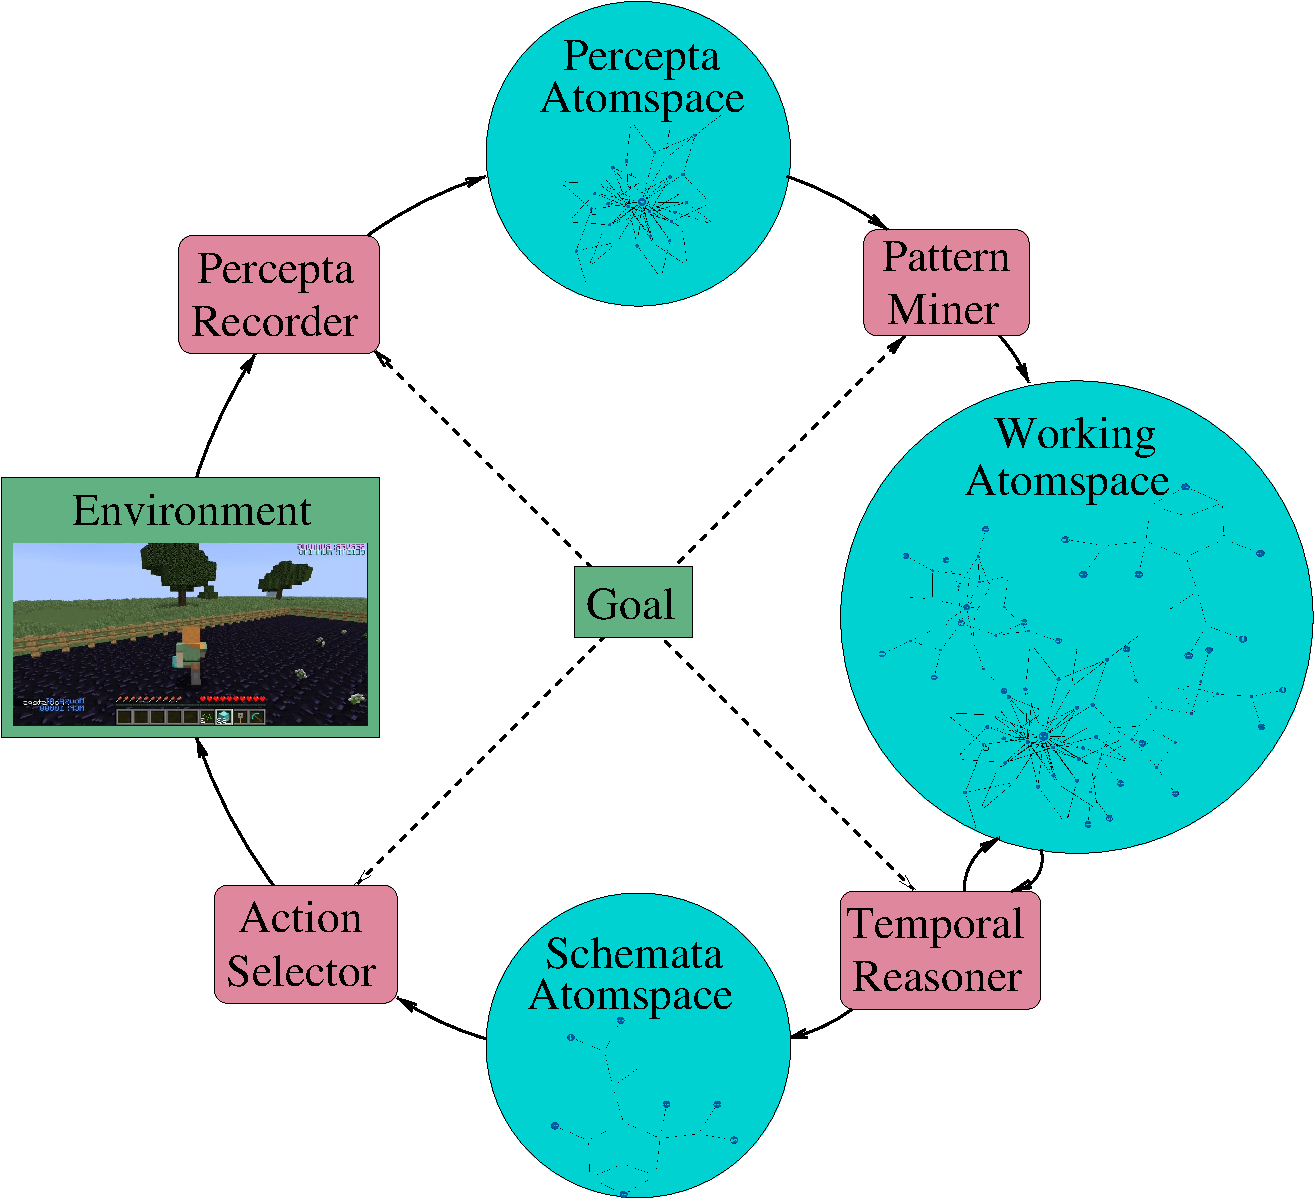
\includegraphics[width=0.54\textwidth]{pictures/rocca-chart-v0.7.pdf}
  \end{center}
  \vspace{-20pt}
  \caption{Rational OpenCog Controlled Agent control and learning
    cycles merged into a single loop.}
  \vspace{-32pt}
  \label{fig:rocca}
\end{wrapfigure}
% \begin{SCfigure}
%   \centering
%   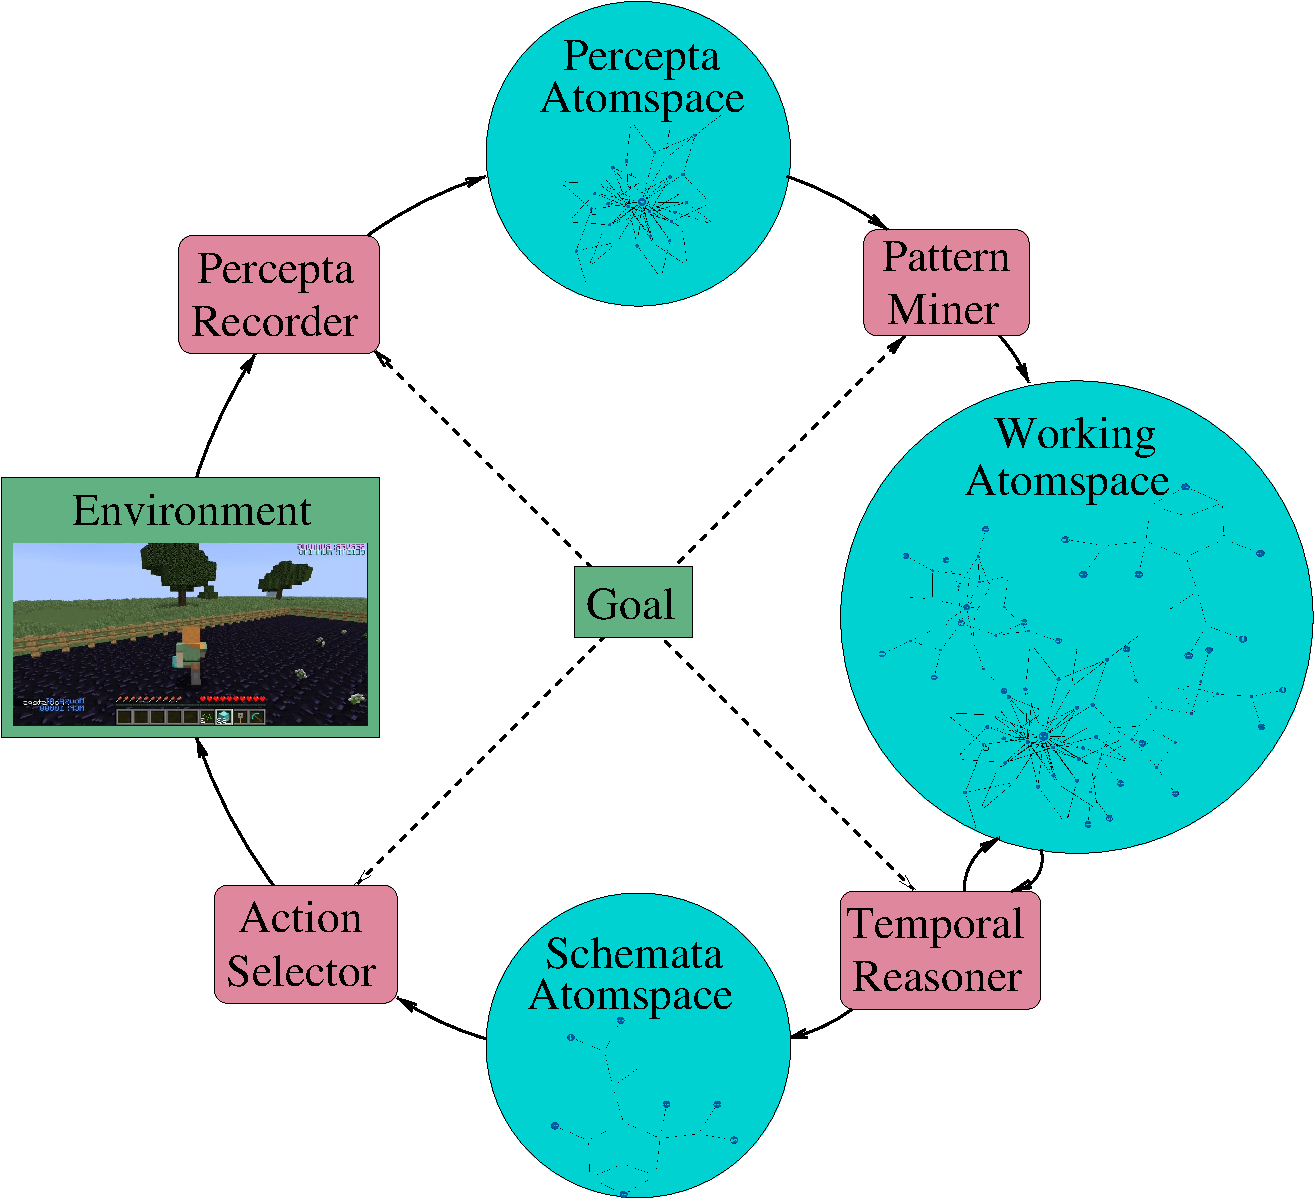
\includegraphics[width=0.6\textwidth]{pictures/rocca-chart-v0.7.pdf}
%   \caption{Rational OpenCog Controlled Agent control and learning
%     cycles merged into a single loop.}
%   \label{fig:rocca}
% \end{SCfigure}
% \begin{figure}
%   \centering
%   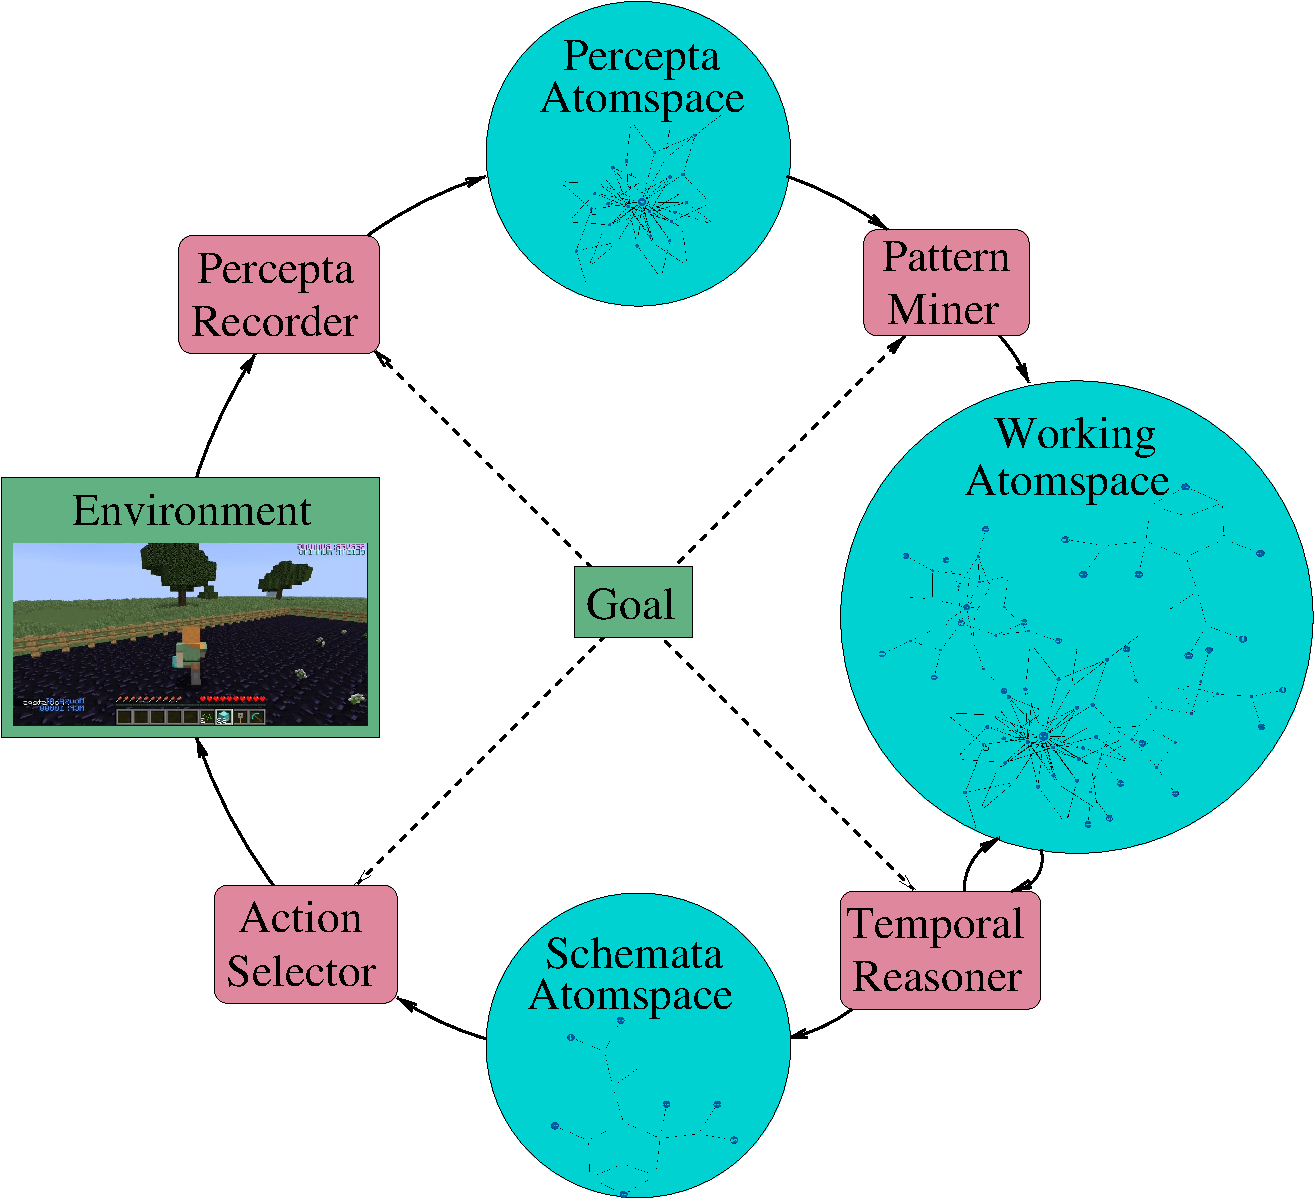
\includegraphics[width=0.6\textwidth]{pictures/rocca-chart-v0.7.pdf}
%   \caption{ROCCA control and learning loops merged into one.}
%   \label{fig:rocca}
% \end{figure}
% To experiment with temporal and procedural reasoning in the context of
% embodied virtual agents in unknown environments we have implemented a
% project called ROCCA, which stands for \emph{Rational OpenCog
%   Controlled Agent}.  ROCCA essentially acts as an interface between
% virtual environments such as Malmo \cite{Johnson2016} or OpenAI Gym
% \cite{Brockman2016} and OpenCog~\cite{Hart2008}.
%% During the life of the
%% agent control and learning phases are alternated to simulate a form of
%% online learning.
% Ideally, the user should just provide a top goal and ROCCA should
% autonomously orchestrates the necessary learning and the planning to
% fulfill that goal.
%% somewhat like a reinforcement learning agent.
% One may possibly see ROCCA as a reinforcement learning agent with the
% particularity that learning and planning are, at least in principle,
% done via reasoning.
% In that respect it is similar in spirit to
% OpenNARS for Applications (ONA)~\cite{Hammer2020} but uses
% PLN~\cite{Goertzel2009} as its core
% reasoning logic rather than NAL~\cite{Wang2011}.\\
%% Where it differs from a typical
%% reinforcement learning agent in that both learning and planning are,

% TODO: explain cognitive schematics

\subsection{Memory}
For better efficiency and clarity, the memory of the agent is split
into three parts.
\begin{enumerate}
\item The \emph{Percepta}
  % ~\footnote{Percepta means percepts in Latin.
  %   It is the plurial form of perceptum.  Latin was chosen over
  %   English so that the difference between singular and plurial does
  %   not reduce to a single letter which can be prone to error when
  %   reading and writing code.}
  AtomSpace holds timestamped
  observations as they come into the system.
\item The \emph{Working} AtomSpace holds any kind of data, ranging
  from timestamped observations to predictive implications.  Most
  knowledge used and inferred during the course of learning are
  usually dumped into this AtomSpace.
\item The \emph{Schemata} AtomSpace holds \emph{Cognitive Schematics},
  which are predictive implications relating contexts, actions and
  goals.%  These may describe how the world work, and may be turned
  %into usable plans as well.
\end{enumerate}
% The reasons for such splitting are:
% \begin{enumerate}
% \item Increased \emph{efficiency}, both the Percepta and Schemata
%   AtomSpaces are specialized to hold only what is required for rapid
%   IO processing.
% \item Increased \emph{clarity}, troubleshooting and repairing is
%   easier that way.
% \end{enumerate}

\subsection{Processes}
% Figure~\ref{fig:rocca} shows a large cycle moving through all phases
% sequentially.  In theory that is valid, but in practice we want to
% split processes, TODO.
The agent runs two main processes:
\begin{enumerate}
\item A \emph{Control} process for real-time reactive agent control.
\item A \emph{Learning} process for non-reactive background learning.
\end{enumerate}
In principle these two processes could happen in parallel.  For now
they alternate in series.  The agent starts in a control phase.  A
number of control cycles occur as the agent motor-babbles through its
environment.  It is then followed by a learning phase when the agent
discover regularities and build plans.  And finally repeats the
control phase to test how it performs after learning.

\subsection{Control}
The control process is composed of control cycles, each decomposed
into \emph{Observation}, \emph{Planning} and \emph{Action} phases, as
described below.
\begin{enumerate}
\item \emph{Observation}:
  \begin{enumerate}
  \item Receive and timestamp observations, reward included, from the
    environment.
  \item Store the timestamped observations in the Percepta AtomSpace.
  \end{enumerate}
\item \emph{Planning}:
  \begin{enumerate}
  \item Select the goal for that cycle.
  \item Find plans fulfilling that goal from the Schemata AtomSpace.
  \item Build a mixture distribution from these plans.
  \end{enumerate}
\item \emph{Action}:
  \begin{enumerate}
  \item Select the next action via Thompson Sampling according to that
    mixture distribution.
  \item Timestamp and store the selected action in the Percepta
    AtomSpace.
  \item Run the selected action and by that update the environment.
  \end{enumerate}
\end{enumerate}
None of these steps are computationally expensive.  They involve
algorithms that are at most linear with the size of the Percepta and
Schemata AtomSpaces.  As time goes and knowledge accumulates though,
it will progressively slow down.  Indeed, for real-time responsiveness
such control cycle should be bound by a constant.  Achieving this may
require to incorporate other mechanisms such as filtering and
forgetting.  This problem, as important as it is, is left aside for
future research. % Discussions about that problem can be found
% in~\cite{Goertzel2014EGI2}.
Given the small environments ROCCA has
been tested with, it has not been a problem so far.
% More on the
% subject of \emph{Attention Allocation} can be found in the Chapter 4
% of~\cite{Goertzel2014EGI2}.
Let us now provide more details about these three phases.

\subsubsection{Observation}
During the observation phase, data coming from the environment are
timestamped and stored in the Percepta AtomSpace with the format
\textit{datum@timestamp}.  For instance if at cycle 3 the agent
observes \textit{outside(house)}, then \textit{outside(house)@3}
% and \textit{hold(key)@3}
% \begin{itemize}
% \item \texttt{outside(house)}
% \item \texttt{hold(key)}
% \end{itemize}
% then
% \begin{itemize}
% \item \texttt{outside(house)@10}
% \item \texttt{hold(key)@10}
% \end{itemize}
% are
is inserted into the Percepta AtomSpace.

\subsubsection{Planning}
The first step of the planning phase is to select a goal $G$ to
fulfill.  In the current version of ROCCA though it merely returns a
constant goal which is to gain a reward within a forward window.  More
on goal selection can be found in~\cite{Goertzel2014EGI1, Hahm2021}.
Once the goal has been selected, the agent searches the Schemata
AtomSpace with the following pattern matcher query
$$\$C \land \$A \lpreimp{T} G$$
where
% \begin{itemize}
% \item $\$C$ is a variable representing the context,
% \item $\$A$ is a variable representing the action or action
%   plan~\footnote{Variables are actually typed so that the pattern
%     matcher cannot confuse what is context and action.},
% \item $T$ is a time delta selected within that forward window,
% \item $G$ is the selected goal.
% \end{itemize}
$\$C$ is a variable representing the context, $\$A$ is a variable
representing the action or action plan~\footnote{Variables are
  actually typed so that the pattern matcher cannot confuse what is
  context and action.}, $T$ is a time delay selected within that
forward window and $G$ is the selected goal.  All returned candidates
are then filtered according to their contexts, only retaining those
for which the context is evaluated to $\TTrue$ at the current time.
Ideally, such crisp evaluation should be replaced by a second order
probability evaluation of a context being $\TTrue$.  This is important
for contexts that have elements of uncertainty.  But for the sake of
simplicity, in our experiments so far, all contexts are crisply
evaluated.  Then from the set of valid cognitive schematics, a second
order mixture distribution is built and handed to the next phase for
performing action selection.  The calculations used to build that
second order mixture distribution is detailed
in~\cite{Geisweiller2018}.
% approximating very roughly a Solomonoff
% distribution as explained in~\cite{Geisweiller2018}.

\subsubsection{Action}
The Action phase consists of the following steps:
\begin{enumerate}
\item Select the next action via Thompson Sampling~\cite{Leike2016}
  according to the mixture distribution built during the planning
  phase.
\item Timestamp and store the selected action in the Percepta
  AtomSpace.
\item Run the selected action and updates the environment.
\end{enumerate}
The trickiest step here is selecting the next action via Thompson
Sampling.  The novelty is that the second order probabilities can be
leveraged by Thompson Sampling.  For example, assume we have two
actions, $A_1$ and $A_2$, to choose among two predictive implications
$$
\begin{array}{c}
  C_1 \land A_1 \lpreimp{T} G \measeq\ <\!0.6, 0.9\!> \\
  C_2 \land A_2 \lpreimp{T} G \measeq\ <\!0.7, 0.1\!>
\end{array}
$$
Using only the strengths of the truth values as proxy for probability
of success, the choice is clear.  Action $A_2$ should be selected,
because its probability of success, which is 0.7, is greater than that
of $A_1$, which is 0.6.  However once confidence is introduced, that
choice becomes less clear because the truth value of success of $A_2$
has a low confidence of 0.1.  In that case, first order probabilities
are sampled from their corresponding second order distributions,
% associated to the truth values of success of $A_1$ and $A_2$,
and then these probabilities are compared.  The action with the
maximum probability gets selected.  Informally, the idea is to
consider the possibilities that the agent might be living in a world
where $A_2$ has a lower probability of success than $A_1$.  That is
the essence of Thompson Sampling.
\begin{figure}
  \centerline{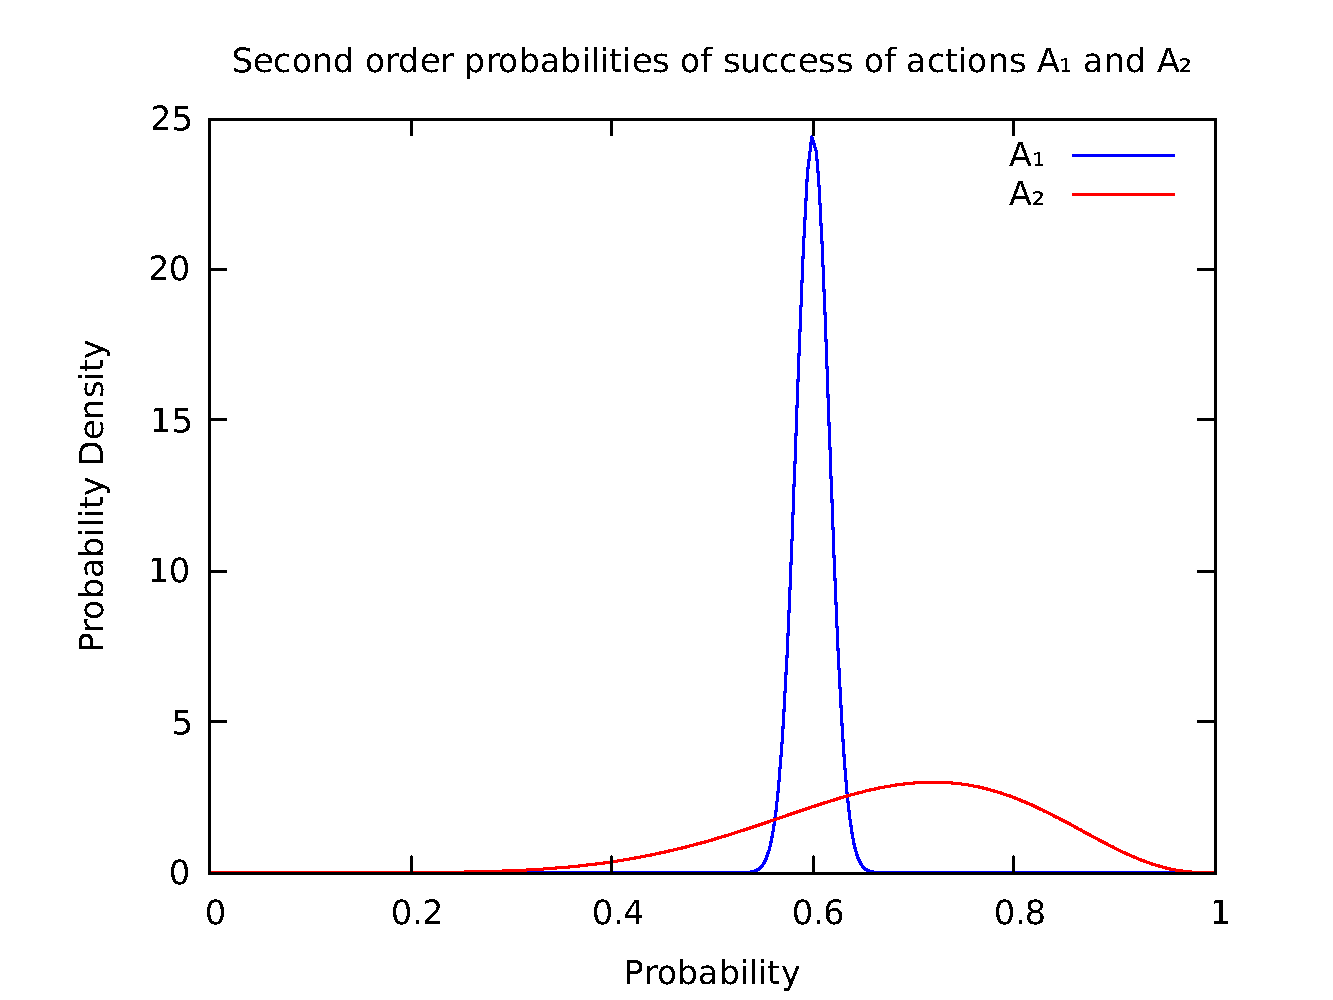
\includegraphics[width=0.8\textwidth]{pictures/actiondist.pdf}}
  \caption{Second order probability distributions of success of
    actions $A_1$ and $A_2$, using as parameters of the beta
    distribution $\alpha(s, c)=\alpha_0 + \frac{s.c.k}{1-c}$ and
    $\beta(s, c)=\beta_0 + \frac{(1-s).c.k}{1-c}$} where $k$, the
  \emph{lookahead}, is set to 100, and $\alpha_0$ and $\beta_0$ are
  set to Jeffreys prior.
  \label{fig:actiondist}
\end{figure}
Figure~\ref{fig:actiondist} shows the second order distributions of
the probabilities of success of $A_1$, in blue, and $A_2$, in red, for
these truth values.  As one may notice, the area under the red curve
situated at the left of the blue curve is non-negligible.  Meaning
that the probability of being in a world where $A_1$ has a higher
probability of success than $A_2$ is non-negligible as well.  Because
these strengths and confidences are periodically updated during the
lifetime of the agent, one can see how Thompson Sampling is a great
alternative to $\varepsilon$-greedy, as it offers a parameter-free
mechanism to balance exploration and exploitation that dynamically
adapts with the knowledge of the agent.

Note that in this example only two actions among two cognitive
schematics are considered, but in practice there is usually a handful
of actions among a potentially very large number of cognitive
schematics with overlapping contexts and conflicting goals.  The
resulting distribution of success of each action is typically
multi-modal and do not reduce to a beta distribution.  How to deal
with such a multitude of cognitive schematics is treated
in~\cite{Geisweiller2018}.

% For that we use a variation of Solomonoff induction described
% in~\cite{Geisweiller2018} which is especially suited for plans
% described by conditional second order distributions, in other words
% predictive implications.  More specifically plans are predictive
% implications of the form
% $$C \land A \lpreimp{T} G \measeq \textit{TV}$$
% called \emph{Cognitive Schematics} or \emph{Schemata}.  Which can be
% read as \emph{``in some context $C$, if some action $A$ is executed,
%   then after $T$ time units, the goal $G$ is likely to be fulfilled,
%   with probability described by $\textit{TV}$''}.  Note that $A$ does
% not need to be limited to elementary actions but can be composite as
% well, potential describing entire plans composed of action sequences,
% conditionals and such, akin to behavior trees.  In other words,
% Cognitive Schematics should be expressive enough for general decision
% making.
% The likelihood of goal fulfillment is specified by the truth
% value of the predictive implication link, which is not indicated in
% that notational format but is present in the extended Atomese format.
% The difficulty then comes down to discovering cognitive schematics
% that are as predictive and widely applicable as possible, which
% translates into predictive implications which broad contexts, high
% strength and high confidence.  An example of an ideal cognitive
% schematic would be
% $$\mathbb{True} \land A \lpreimp{T} G \measeq\ <\! 1, 1\! >$$
% that has a strength and confidence of one, and is universally
% applicable\footnote{$\mathbb{True}$ represents the predicate that is
%   always true}.  For real environments and goals however, such ideal
% is beyond reach.  More often than not we will have instead a large
% collection of cognitive schematics with narrow contexts and poor
% predictiveness.  To make the best of it, a mixture of second order
% distributions is built over all applicable cognitive schematics, in a
% manner that approximates a Solomonoff distribution, as described
% in~\cite{Geisweiller2018}.  Action selection is then performed based
% on that mixture using Thompson Sampling~\cite{Leike2016}.
% , and
% excellent at balancing exploitation and exploration in principle.

\subsection{Learning}
The difficulty then comes down to discovering cognitive schematics
that are as predictive and widely applicable as possible.  For that,
ROCCA uses a combination of pattern mining and reasoning.
% This
% translates into predictive implications which broad contexts, high
% strength and high confidence.
% As hinted above, the ultimate goal of the learning phase is to
% discover maximally useful cognitive schematics, and by useful it is
% specifically meant that they are as predictive and cover as many cases
% as possible.

\subsubsection{Pattern Mining}
A relatively inexpensive way to discover regularities in the
environment is to mine the Percepta AtomSpace.  For instance, given
$$\{\textit{go(right)@0},\ \textit{square(right)@1},\
\textit{go(left)@1},\ \textit{square(left)@2}, \dots\}$$ the pattern
miner can discover temporal relationships such as
$$
\begin{array}{c}
  \lgo{\textit{right}} \lpreimp{1} square(right) \\
  \lgo{\textit{left}} \lpreimp{1} square(left)
\end{array}
$$
as well as more abstract relationships, such as
$$\lgo{x} \lpreimp{1} square(x)$$
The pattern mining algorithm used by ROCCA is detailed
in~\cite{Geisweiller2019}.  This is a generic hypergraph pattern
miner, not specialized for temporal patterns.  In order to mine
temporal patterns with it, timestamps are represented as naturals.  0
is presented by $Z$, 1 by $S(Z)$, 2 by $S(S(Z))$, etc.  This provides
the needed structure to discover temporal relationships between
events.  As it currently stands, the pattern miner can efficiently
discover mono-action plans.  Mining poly-action plans is also possible
but has two issues:
\begin{enumerate}
\item In the worse case, the computational cost of mining goes up
  exponentially with the size of the action sequence to mine.
\item The number of observations to accumulate in order to generate
  cognitive schematics with decent confidences goes up exponentially
  as well.
\end{enumerate}
The latter is really the most problematic because we cannot buy our
way out of it.  If each observation takes a certain amount time,
determined by the control cycle period in the case of primary
observations, then we have to go through them, we cannot speed time
up.  This is even more true for abstract percepta that can only be
observed at periods that are multiples of control cycle periods.
Also, in some cases, a particular action sequence may never be
observed at all, yet we still would like to have a way to estimate the
likelihood of its success.  In order to address these limitations and
more, we need reasoning.

\subsubsection{Temporal Reasoning}
ROCCA uses a temporal extension of PLN described
in~\cite{Geisweiller2023TPLN} to update existing cognitive schematics
obtained by pattern mining, and discover new cognitive schematics by
combining existing ones.  For instance it can infer poly-action plans
by stringing mono-action plans together, as well as generalize or
specialize their contexts or goals.  Temporal rules integrated into
ROCCA include:
\begin{enumerate}
\item \emph{Predictive Implication Direct Introduction} to infer the
  truth value of a predictive implication from direct observations.
\item \emph{Temporal Conditional Conjunction Introduction} to
  specialize a goal within a plan by considering the conjunction of
  existing cognitive schematics goals.
\item \emph{Temporal Deduction} to string together small plans to form
  bigger ones.
\end{enumerate}
The precise semantics of these rules is detailed
in~\cite{Geisweiller2023TPLN}.  An example of how they are used is
presented below.
% in Section~\ref{sec:minecraft}.

\section{Experiment in a Simple Minecraft Environment}
\label{sec:minecraft}
In this experiment, we use Malmo [15] to construct a basic Minecraft
world that comprises a house filled with diamonds and a key. The
objective of the agent is to locate the key, which is placed somewhere
in the proximity of the house, retrieve it, and then unlock the door
of the house. Upon unlocking the door, the agent is able to collect a
diamond and receive a reward. \par
The aim of the experiment is to make ROCCA learn from interacting
% its actions and
% perceptions
with the Minecraft environment
% so as to be able
and collect as many diamonds as possible.
% The ROCCA agent performs a series of possible
% actions with a goal of achieving a reward and learns from them by
% applying PLN and Pattern Miner.
To make the task easier, the primary actions and perceptions provided
by Malmo have been replaced by high level actions
% and perceptions
% where details have been abstracted away.
%Thus we have implemented
%actions
such as \textit{go(key)}, \textit{go(house)} and
\textit{go(diamonds)}, as well as high level perceptions about the
state of the agent such as \textit{outside(house)}, \textit{hold(key)}
and the reward for completing a given action, \textit{reward(1)}. \par
% We conducted various experiments by adjusting different parameters.
The experiment consists of two iterations of training lasting fifty
control cycles each, interleaved by a learning phase lasting an
hour. During the first iteration, no learning is taking place as the
agent has no prior knowledge. The agent randomly explores the
environment. Then it enters a learning phase, discovering cognitive
schematics via mining and reasoning, subsequently leading the agent to
achieve more frequently its goal during the next training phase.

% \subsubsection{Experimental result}

Let us look more closely how ROCCA discovers cognitive
schematics. Given the following observations
% during the second learning-training cycle
$$
\begin{array}{l}
\{\textit{Reward(0)@50},\ \textit{outside(house)@50},\
\textit{hold(key)@50},\ \textit{go(house)@50},\\ \ \textit{inside(house)@51},\ \textit{go(diamond)@51},\ \textit{Reward(0)@51},\ \textit{Reward(1)@52}, \dots\}
\end{array}
$$
ROCCA can mine, among many others, the following cognitive schematic
% through the Pattern Miner and infer their truth value using the Predictive Implication rule.
$$
\textit{hold(key)} \land \textit{go(house)} \lpreimp{1} \textit{inside(house)} \measeq\ <\!0.833, 0.007\!>
$$
Additionally, by applying the temporal conditional conjunction
introduction rule on the relevant relationships, such as
$$
\begin{array}{l}
\textit{outside(house)} \land \textit{go(key)} \lpreimp{1} \textit{outside(house)} \measeq\ <\!1, 0.007\!> \\
\textit{outside(house)} \land \textit{go(key)} \lpreimp{1} \textit{hold(key)} \measeq\ <\!1, 0.007\!>
\end{array}
$$
the agent derives
$$\textit{outside(house)} \land \textit{go(key)} \lpreimp{1}
\textit{outside(house)} \land \textit{hold(key)} \measeq\ <\!1, 0.007\!>$$
which, if combined with
$$\textit{hold(key)} \land \textit{outside(house)} \land \textit{go(house)} \lpreimp{1} \textit{inside(house)} \measeq\ <\!0.833, 0.007\!>$$
can be used by the procedural deduction rule to infer
$$\textit{outside(house)} \land \textit{go(key)} \lseqand{1} \textit{go(house)} \lpreimp{2} \textit{inside(house)} \measeq\ <\!0.833, 0.007\!>$$
% $$
% \textit{Reward(0)} \land \textit{inside(house)} \land \textit{go(diamond)} \lpreimp{1} \textit{Reward(1)} \measeq\ <\!1, 0.006\!>
% $$
Continuing this reasoning process ultimately results in the discovery
of an effective plan that leads to achieving the goal, such as
{\small
$$\textit{outside(house)} \land \textit{go(key)} \lseqand{1}
\textit{go(house)} \lseqand{1} \textit{go(diamond)} \lpreimp{3}
\textit{inside(house)} \measeq\ <\!0.833, 0.005\!>$$ }
% $$
% \begin{small}
% \textit{hold(key)} \land \textit{outside(house)} \land \textit{go(house)} \lseqand{T} \textit{go(diamond)} \lpreimp{T+1} \textit{Reward(1)} \measeq\ <\!0.833, 0.005\!>
% \end{small}
% $$
We evaluate the agent's performance based on two factors: the
cognitive schematics it has learned and the rewards it has
accumulated. Our results indicate that ROCCA successfully learned the
necessary cognitive schematics and accumulates substantially more
rewards in the second iteration.  Incidentally, one may notice that
some plans are not completely reliable, their strengths is below 1.
That is because some actions may fail.  ROCCA has no problem with that
and is perfectly suited for dealing with such uncertainty.  All in all
however, these findings only apply to a very simple Minecraft
environment
% with a limited
% number of actions
and may not be indicative of the overall performance of ROCCA.  More
experiments over more environments are required
% to draw definitive conclusions about its performance,
and will be pursued in future work.  A video of this experiment is
available on YouTube~\cite{ROCCADemo}.

\section{Conclusion}
\label{sec:conclusion}
A system called ROCCA, that leverages the OpenCog framework for
controlling an agent in uncertain environments has been presented.
This agent is in a strong sense fully reasoning-based, from learning
to planning.  The advantage we believe of such approach, in spite of
its current inefficiencies, is to offer greater transparency and
foster greater capabilities for meta-learning and self-improvement.
As such, we are only at the start of our endeavor.  Towards that end,
future directions include:
\begin{enumerate}
% \item Support temporal intervals and scales and add more temporal, as
%   well as spatial inference rules.
\item Integrate \emph{Economic Attention Networks}~\cite{Pitt2009} for
  \emph{Attention Allocation}.  Record attentional spreading as
  percepta to learn Hebbian links~\cite{Pitt2009} and improve
  attention allocation in return.
\item Carry out concept creation and schematization, also called
  crystallized attention allocation, to speed up repetitive
  information processing.  This done well should also provide a
  solution to the problem of creating hierarchies of abstract
  observations and actions.
\item Record more internal processes, not just attentional spreading, as
  internal percepta to enable deeper forms of introspection.
\item Plan with internal actions, not just external, such as parameter
  fine-tuning and code rewriting to enable self-improvements.
\end{enumerate}

% \begin{enumerate}
% \item Forgetting
% \item Functional Pattern Mining
% \item Attention Allocation
% \item Inner actions
% \item Port to OpenCog Hyperon
% \item Higher level percepts
% \item Second order evaluation of context being currently true
% \item Time interval
% \end{enumerate}

%
% ---- Bibliography ----
%
\bibliographystyle{splncs04} \bibliography{local}

\end{document}
